Let us assume a Cartesian domain discretised in $nel_x \times nel_y$
elements in 2D and $nel_x \times nel_y \times nel_z$ elements in 3D.
Focusing only on the total number of velocity dofs (the values indicated after the 
arrows are the limits when $nel_x=nel_y=nel_z >> 1$):

\begin{itemize}

\item $Q_1 \times P_0$, $Q_1 \times Q_1$
\begin{align}
ndof_{2D}&= 2 (nel_x+1) \cdot (nel_y+1) 
& \rightarrow  2 \cdot nel_x^2   \\
ndof_{3D}&= 3 (nel_x+1) \cdot (nel_y+1) \cdot (nel_z+1)
& \rightarrow 3 \cdot nel_x^3 
\end{align}

\item $Q_2 \times P_{-1}$, $Q_2 \times Q_1$
\begin{eqnarray}
ndof_{2D}      &=&2 (2nel_x+1) \cdot (2nel_y+1) 
\qquad \rightarrow \qquad 8 \cdot nel_x^2   \nonumber\\
ndof_{3D}&=&3 (2nel_x+1) \cdot (2nel_y+1) \cdot (2nel_z+1)
\qquad \rightarrow \qquad 24 \cdot nel_x^3 \nonumber
\end{eqnarray}


\item $Q_1^+ \times P_0$

\begin{eqnarray}
ndof_{2D}     &=&2 (nel_x+1) \cdot (nel_y+1) + (nel_x+1)\cdot nel_y + nel_x\cdot(nel_y+1)
\qquad \rightarrow \qquad 4 \cdot nel_x^2   \nonumber\\
ndof_{3D}&=&3 (nel_x+1) \cdot (nel_y+1) \cdot (nel_z+1) \nonumber\\
&+&  (nel_x+1)\cdot nel_y \cdot nel_z + nelx\cdot (nel_y+1) \cdot nelz + nelx\cdot nely \cdot (nel_z+1)
\quad \rightarrow \quad 6 \cdot nel_x^3 \nonumber
\end{eqnarray}

\item $Q_1 \times Q_1$+1 bubble

\begin{eqnarray}
ndof_{2D}&=& 2[(nel_x+1) \cdot (nel_y+1)  + \cdot nelx\cdot nely ]
\quad \rightarrow \quad 4 \cdot nel_x^2 \nonumber
\end{eqnarray}

%\item $Q_1^+ \times Q_1$
%\begin{eqnarray}
%ndof_{2D}  &=&2 [ (nel_x+1) \cdot (nel_y+1) + nel_x \cdot nel_y ]
%\qquad \rightarrow \qquad 4 \cdot nel_x^2   \nonumber
%ndof_{3D}  &=&3 [ (nel_x+1) \cdot (nel_y+1) \cdot (nel_z+1) + nel_x \cdot nel_y \cdot nel_z ]
%\qquad \rightarrow \qquad 6 \cdot nel_x^3 \nonumber
%\end{eqnarray}

\item $Q_1 \times Q_1$+2 bubbles

\begin{eqnarray}
ndof_{3D}&=& 3[(nel_x+1) \cdot (nel_y+1) \cdot  (nel_z+1) + 2\cdot nelx\cdot nely \cdot nelz]
\quad \rightarrow \quad 9 \cdot nel_x^3 \nonumber
\end{eqnarray}


\item Rannacher-turek or DSSY:

\begin{eqnarray}
ndof_{2D}&=& 2[(nel_y+1) \cdot nel_x+nel_y\cdot(nel_x+1)  ] 
\quad\rightarrow \quad 4 \cdot nel_x^2 \nonumber\nn\\
ndof_{3D}&=& 3[ nel_x\cdot (nel_y+1)\cdot nel_z + (nel_x+1) \cdot nel_y\cdot nel_z  +nel_x\cdot nel_y\cdot (nel_z+1) ]  
\quad \rightarrow \quad 9 \cdot nel_x^3 \nonumber
\end{eqnarray}
 

\end{itemize}


If we now assume $nel_x=nel_y=nel_z$, we can then plot the values above as a function of $nel_x$:
\begin{center}
\includegraphics[width=7.5cm]{images/elements/ndof2D.pdf}
\includegraphics[width=7.5cm]{images/elements/ndof3D.pdf}
\end{center}

We see that the $Q_1^+\times Q_1$ and $Q_1^+ \times P_0$ actually 
yield the same number of velocity dofs. 

Simply based on the dof count and wishing for a (bi/tri)linear approximation 
for pressure, we must conclude that the $Q_1\times Q_1$+2 bubbles is the most desirable 
since it is also LBB stable.

\begin{center}
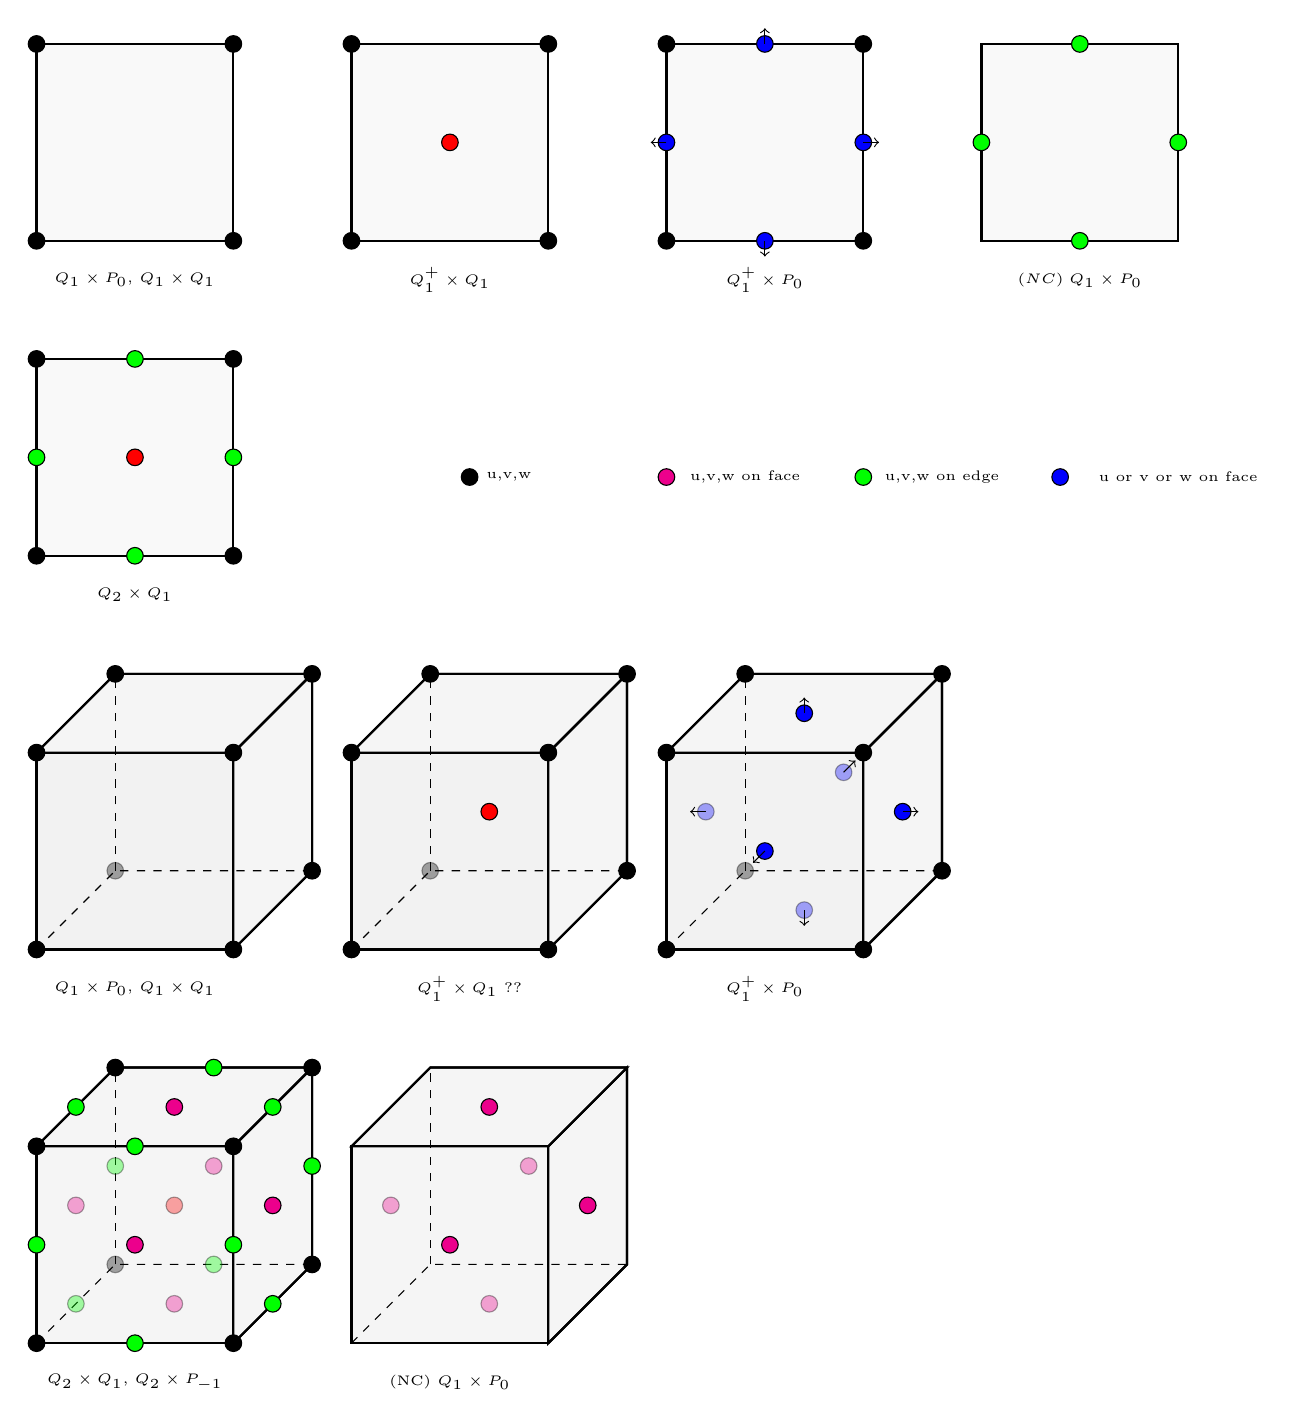
\begin{tikzpicture}
%\draw[fill=gray!23,gray!23](0,0) rectangle (20,10);
%\draw[step=0.5cm,gray,very thin] (0,0) grid (18,18); %background grid

%%%%%%%%%%%%%%%%%%%%%%%%%%%%%%%%%%%%%%%%%%%%%%%%%%%%%%%%%%%%%%%%%%%%
%bottom row
%%%%%%%%%%%%%%%%%%%%%%%%%%%%%%%%%%%%%%%%%%%%%%%%%%%%%%%%%%%%%%%%%%%%
\draw[thick,fill=gray!8] (1,1) -- (3.5,1) -- (3.5,3.5) -- (1,3.5) -- cycle;
\draw[thick,fill=gray!8] (5,1) -- (7.5,1) -- (7.5,3.5) -- (5,3.5) -- cycle;
%\draw[thick,fill=gray!8] (9,1) -- (11.5,1) -- (11.5,3.5) -- (9,3.5) -- cycle;
%\draw[thick,fill=gray!8] (13,1) -- (15.5,1) -- (15.5,3.5) -- (13,3.5) -- cycle;

%right sides
\draw[thick,fill=gray!8] (3.5,1) -- (4.5,2) -- (4.5,4.5) -- (3.5,3.5) -- cycle;
\draw[thick,fill=gray!8] (7.5,1) -- (8.5,2) -- (8.5,4.5) -- (7.5,3.5) -- cycle;
%\draw[thick,fill=gray!8] (11.5,1) -- (12.5,2) -- (12.5,4.5) -- (11.5,3.5) -- cycle;
%\draw[thick,fill=gray!8] (15.5,1) -- (16.5,2) -- (16.5,4.5) -- (15.5,3.5) -- cycle;

%tops
\draw[thick,fill=gray!8] (1,3.5) -- (3.5,3.5) -- (4.5,4.5) -- (2,4.5) -- cycle;
\draw[thick,fill=gray!8] (5,3.5) -- (7.5,3.5) -- (8.5,4.5) -- (6,4.5) -- cycle;
%\draw[thick,fill=gray!8] (9,3.5) -- (11.5,3.5) -- (12.5,4.5) -- (10,4.5) -- cycle;
%\draw[thick,fill=gray!8] (13,3.5) -- (15.5,3.5) -- (16.5,4.5) -- (14,4.5) -- cycle;

\draw[thick] (1,3.5) -- (2,4.5) -- (4.5,4.5) -- (4.5,2) -- (3.5,1);
\draw[thick] (5,3.5) -- (6,4.5) -- (8.5,4.5) -- (8.5,2) -- (7.5,1);
%\draw[thick] (9,3.5) -- (10,4.5) -- (12.5,4.5) -- (12.5,2) -- (11.5,1);
%\draw[thick] (13,3.5) -- (14,4.5) -- (16.5,4.5) -- (16.5,2) -- (15.5,1);

\draw[thick] (3.5,3.5) -- (4.5,4.5) ;
\draw[thick] (7.5,3.5) -- (8.5,4.5) ;
%\draw[thick] (11.5,3.5) -- (12.5,4.5) ;
%\draw[thick] (15.5,3.5) -- (16.5,4.5) ;

\draw[dashed] (1,1) -- (2,2) -- (4.5,2) ;\draw[dashed] (2,2) -- (2,4.5);
\draw[dashed] (5,1) -- (6,2) -- (8.5,2) ;\draw[dashed] (6,2) -- (6,4.5);
%\draw[dashed] (9,1) -- (10,2) -- (12.5,2) ;\draw[dashed] (10,2) -- (10,4.5);
%\draw[dashed] (13,1) -- (14,2) -- (16.5,2) ;\draw[dashed] (14,2)--(14,4.5);

\draw[black,fill=black] (1,1)   circle (3pt);
\draw[black,fill=black] (3.5,1)   circle (3pt);
\draw[black,fill=black] (3.5,3.5)   circle (3pt);
\draw[black,fill=black] (1,3.5)   circle (3pt);
\draw[black,fill=black] (2,4.5)   circle (3pt);
\draw[black,fill=black] (4.5,4.5)   circle (3pt);
\draw[black,fill=black] (4.5,2)   circle (3pt);
\draw[black,fill=black,opacity=0.35] (2,2)   circle (3pt);

%\draw[black,fill=black] (5,1)   circle (3pt);
%\draw[black,fill=black] (7.5,1)   circle (3pt);
%\draw[black,fill=black] (7.5,3.5)   circle (3pt);
%\draw[black,fill=black] (5,3.5)   circle (3pt);
%\draw[black,fill=black] (6,4.5)   circle (3pt);
%\draw[black,fill=black] (8.5,4.5)   circle (3pt);
%\draw[black,fill=black] (8.5,2)   circle (3pt);
%\draw[black,fill=black,opacity=0.35] (6,2)   circle (3pt);

%\draw[black,fill=black] (9,1)   circle (3pt);
%\draw[black,fill=black] (11.5,1)   circle (3pt);
%\draw[black,fill=black] (11.5,3.5)   circle (3pt);
%\draw[black,fill=black] (9,3.5)   circle (3pt);
%\draw[black,fill=black] (10,4.5)   circle (3pt);
%\draw[black,fill=black] (12.5,4.5)   circle (3pt);
%\draw[black,fill=black] (12.5,2)   circle (3pt);
%\draw[black,fill=black,opacity=0.35] (10,2)   circle (3pt);

%\draw[black,fill=black] (13,1)   circle (3pt);
%\draw[black,fill=black] (15.5,1)   circle (3pt);
%\draw[black,fill=black] (15.5,3.5)   circle (3pt);
%\draw[black,fill=black] (13,3.5)   circle (3pt);
%\draw[black,fill=black] (14,4.5)   circle (3pt);
%\draw[black,fill=black] (16.5,4.5)   circle (3pt);
%\draw[black,fill=black] (16.5,2)   circle (3pt);
%\draw[black,fill=black,opacity=0.35] (14,2)   circle (3pt);


%%%%%%%%%%%%%%%%%%%%%%%%%%%%%%%%%%%%%%%%%%%%%%%%%%%%%%%%%%%%%%%%%%%%
%3rd row 
%%%%%%%%%%%%%%%%%%%%%%%%%%%%%%%%%%%%%%%%%%%%%%%%%%%%%%%%%%%%%%%%%%%%

\draw[thick,fill=gray!5] (1,15) -- (3.5,15) -- (3.5,17.5) -- (1,17.5) -- cycle;
\draw[thick,fill=gray!5] (5,15) -- (7.5,15) -- (7.5,17.5) -- (5,17.5) -- cycle;
\draw[thick,fill=gray!5] (9,15) -- (11.5,15) -- (11.5,17.5) -- (9,17.5) -- cycle;
\draw[thick,fill=gray!5] (13,15) -- (15.5,15) -- (15.5,17.5) -- (13,17.5) -- cycle;

\draw[black,fill=black] (1,15)   circle (3pt);
\draw[black,fill=black] (3.5,15)   circle (3pt);
\draw[black,fill=black] (1,17.5)   circle (3pt);
\draw[black,fill=black] (3.5,17.5)   circle (3pt);
\node[] at (2.25,14.5) {\tiny $Q_1\times P_0$, $Q_1\times Q_1$};


\draw[black,fill=black] (5,15)   circle (3pt);
\draw[black,fill=black] (7.5,15)   circle (3pt);
\draw[black,fill=black] (5,17.5)   circle (3pt);
\draw[black,fill=black] (7.5,17.5)   circle (3pt);
\node[] at (6.25,14.5) {\tiny $Q_1^+\times Q_1$};
\draw[black,fill=red] (6.25,16.25)   circle (3pt);

\draw[black,fill=black] (9,15)   circle (3pt);
\draw[black,fill=black] (11.5,15)   circle (3pt);
\draw[black,fill=black] (9,17.5)   circle (3pt);
\draw[black,fill=black] (11.5,17.5)   circle (3pt);
\node[] at (10.25,14.5) {\tiny $Q_1^+\times P_0$};

\draw[black,fill=blue] (9,16.25)   circle (3pt);
\draw[black,fill=blue] (11.5,16.25)   circle (3pt);
\draw[black,fill=blue] (10.25,15)   circle (3pt);
\draw[black,fill=blue] (10.25,17.5)   circle (3pt);

\draw[fill=blue,->] (9,16.25) -- (8.8,16.25); 
\draw[fill=blue,->] (11.5,16.25) -- (11.7,16.25); 
\draw[fill=blue,->] (10.25,15) -- (10.25,14.8); 
\draw[fill=blue,->] (10.25,17.5) -- (10.25,17.7); 


\draw[black,fill=green] (14.25,15)   circle (3pt);
\draw[black,fill=green] (14.25,17.5)   circle (3pt);
\draw[black,fill=green] (13,16.25)   circle (3pt);
\draw[black,fill=green] (15.5,16.25)   circle (3pt);
\node[] at (14.25,14.5) {\tiny $(NC)\; Q_1\times P_0$};

%%%%%%%%%%%%%%%%%%%%%%%%%%%%%%%%%%%%%%%%%%%%%%%%%%%%%%%%%%%%%%%%%%%%
%2nd row 
%%%%%%%%%%%%%%%%%%%%%%%%%%%%%%%%%%%%%%%%%%%%%%%%%%%%%%%%%%%%%%%%%%%%

\draw[thick,fill=gray!5] (1,11) -- (3.5,11) -- (3.5,13.5) -- (1,13.5) -- cycle;
%\draw[thick,fill=gray!5] (5,11) -- (7.5,11) -- (7.5,13.5) -- (5,13.5) -- cycle;
%\draw[thick,fill=gray!5] (9,11) -- (11.5,11) -- (11.5,13.5) -- (9,13.5) -- cycle;
%\draw[thick,fill=gray!5] (13,11) -- (15.5,11) -- (15.5,13.5) -- (13,13.5) -- cycle;

\draw[black,fill=black] (1,11)   circle (3pt);
\draw[black,fill=green] (2.25,11)   circle (3pt);
\draw[black,fill=black] (3.5,11)   circle (3pt);
\draw[black,fill=green] (1,12.25)   circle (3pt);
\draw[black,fill=red] (2.25,12.25)   circle (3pt);
\draw[black,fill=green] (3.5,12.25)   circle (3pt);
\draw[black,fill=black] (1,13.5)   circle (3pt);
\draw[black,fill=green] (2.25,13.5)   circle (3pt);
\draw[black,fill=black] (3.5,13.5)   circle (3pt);
\node[] at (2.25,10.5) {\tiny $Q_2\times Q_1$};



%%%%%%%%%%%%%%%%%%%%%%%%%%%%%%%%%%%%%%%%%%%%%%%%%%%%%%%%%%%%%%%%%%%%
%1st row 
%%%%%%%%%%%%%%%%%%%%%%%%%%%%%%%%%%%%%%%%%%%%%%%%%%%%%%%%%%%%%%%%%%%%
\draw[thick,fill=gray!10] (1,6) -- (3.5,6) -- (3.5,8.5) -- (1,8.5) -- cycle;
\draw[thick,fill=gray!10] (5,6) -- (7.5,6) -- (7.5,8.5) -- (5,8.5) -- cycle;
\draw[thick,fill=gray!10] (9,6) -- (11.5,6) -- (11.5,8.5) -- (9,8.5) -- cycle;
%\draw[thick,fill=gray!10] (13,6) -- (15.5,6) -- (15.5,8.5) -- (13,8.5) -- cycle;

%right sides
\draw[thick,fill=gray!8] (3.5,6) -- (4.5,7) -- (4.5,9.5) -- (3.5,8.5) -- cycle;
\draw[thick,fill=gray!8] (7.5,6) -- (8.5,7) -- (8.5,9.5) -- (7.5,8.5) -- cycle;
\draw[thick,fill=gray!8] (11.5,6) -- (12.5,7) -- (12.5,9.5) -- (11.5,8.5) -- cycle;
%\draw[thick,fill=gray!8] (15.5,6) -- (16.5,7) -- (16.5,9.5) -- (15.5,8.5) -- cycle;

%tops
\draw[thick,fill=gray!8] (1,8.5) -- (3.5,8.5) -- (4.5,9.5) -- (2,9.5) -- cycle;
\draw[thick,fill=gray!8] (5,8.5) -- (7.5,8.5) -- (8.5,9.5) -- (6,9.5) -- cycle;
\draw[thick,fill=gray!8] (9,8.5) -- (11.5,8.5) -- (12.5,9.5) -- (10,9.5) -- cycle;
%\draw[thick,fill=gray!8] (13,8.5) -- (15.5,8.5) -- (16.5,9.5) -- (14,9.5) -- cycle;


\draw[thick] (1,8.5) -- (2,9.5) -- (4.5,9.5) -- (4.5,7) -- (3.5,6);
\draw[thick] (5,8.5) -- (6,9.5) -- (8.5,9.5) -- (8.5,7) -- (7.5,6);
\draw[thick] (9,8.5) -- (10,9.5) -- (12.5,9.5) -- (12.5,7) -- (11.5,6);
%\draw[thick] (13,8.5) -- (14,9.5) -- (16.5,9.5) -- (16.5,7) -- (15.5,6);

\draw[thick] (3.5,8.5) -- (4.5,9.5) ;
\draw[thick] (7.5,8.5) -- (8.5,9.5) ;
\draw[thick] (11.5,8.5) -- (12.5,9.5) ;
%\draw[thick] (15.5,8.5) -- (16.5,9.5) ;

\draw[dashed] (1,6) -- (2,7) -- (4.5,7)    ;\draw[dashed] (2,7) -- (2,9.5);
\draw[dashed] (5,6) -- (6,7) -- (8.5,7)    ;\draw[dashed] (6,7) -- (6,9.5);
\draw[dashed] (9,6) -- (10,7) -- (12.5,7)  ;\draw[dashed] (10,7) -- (10,9.5);
%\draw[dashed] (13,6) -- (14,7) -- (16.5,7) ;\draw[dashed] (14,7) -- (14,9.5);

\draw[black,fill=black] (1,6)   circle (3pt);
\draw[black,fill=black] (3.5,6)   circle (3pt);
\draw[black,fill=black] (3.5,8.5)   circle (3pt);
\draw[black,fill=black] (1,8.5)   circle (3pt);
\draw[black,fill=black] (2,9.5)   circle (3pt);
\draw[black,fill=black] (4.5,9.5)   circle (3pt);
\draw[black,fill=black] (4.5,7)   circle (3pt);
\draw[black,fill=black,opacity=0.35] (2,7)   circle (3pt);

\draw[black,fill=black] (5,6)   circle (3pt);
\draw[black,fill=black] (7.5,6)   circle (3pt);
\draw[black,fill=black] (7.5,8.5)   circle (3pt);
\draw[black,fill=black] (5,8.5)   circle (3pt);
\draw[black,fill=black] (6,9.5)   circle (3pt);
\draw[black,fill=black] (8.5,9.5)   circle (3pt);
\draw[black,fill=black] (8.5,7)   circle (3pt);
\draw[black,fill=black,opacity=0.35] (6,7)   circle (3pt);

\draw[black,fill=black] (9,6)   circle (3pt);
\draw[black,fill=black] (11.5,6)   circle (3pt);
\draw[black,fill=black] (11.5,8.5)   circle (3pt);
\draw[black,fill=black] (9,8.5)   circle (3pt);
\draw[black,fill=black] (10,9.5)   circle (3pt);
\draw[black,fill=black] (12.5,9.5)   circle (3pt);
\draw[black,fill=black] (12.5,7)   circle (3pt);
\draw[black,fill=black,opacity=0.35] (10,7)   circle (3pt);

%\draw[black,fill=black] (13,5)   circle (2pt);
%\draw[black,fill=black] (15.5,5)   circle (2pt);
%\draw[black,fill=black] (15.5,7.5)   circle (2pt);
%\draw[black,fill=black] (13,7.5)   circle (2pt);
%\draw[black,fill=black] (14,8.5)   circle (2pt);
%\draw[black,fill=black] (16.5,8.5)   circle (2pt);
%\draw[black,fill=black] (16.5,6)   circle (2pt);
%\draw[black,fill=black,opacity=0.35] (14,6)   circle (2pt);


\node[] at (2.25,5.5) {\tiny $Q_1\times P_0$, $Q_1\times Q_1$};


\node[] at (6.5,5.5) {\tiny $Q_1^+\times Q_1$ ??};
\draw[black,fill=red] (6.75,7.75)   circle (3pt);

\node[] at (10.25,5.5) {\tiny $Q_1^+\times P_0$};
\draw[black,fill=blue,opacity=0.35] (9.5,7.75)   circle (3pt);
\draw[black,fill=blue] (12,7.75)   circle (3pt);
\draw[black,fill=blue,opacity=0.35] (10.75,6.5)   circle (3pt);
\draw[black,fill=blue] (10.75,9)   circle (3pt);
\draw[black,fill=blue] (10.25,7.25)   circle (3pt);
\draw[black,fill=blue,opacity=0.35] (11.25,8.25)   circle (3pt);

\draw[fill=blue,->] (9.5,7.75) -- (9.3,7.75); 
\draw[fill=blue,->] (12,7.75) -- (12.2,7.75); 
\draw[fill=blue,->] (10.75,6.5) -- (10.75,6.3); 
\draw[fill=blue,->] (10.75,9) -- (10.75,9.2); 
\draw[fill=blue,->] (10.25,7.25)  -- (10.1,7.1) ;
\draw[fill=blue,->] (11.25,8.25)  -- (11.4,8.4) ;

\node[] at (2.25,0.5) {\tiny $Q_2\times Q_1$, $Q_2\times P_{-1}$};

\draw[black,fill=red,opacity=0.35] (2.75,2.75)   circle (3pt);

\draw[black,fill=magenta,opacity=0.35] (1.5,2.75)   circle (3pt);
\draw[black,fill=magenta] (4,2.75)   circle (3pt);
\draw[black,fill=magenta,opacity=0.35] (2.75,1.5)   circle (3pt);
\draw[black,fill=magenta] (2.75,4)   circle (3pt);
\draw[black,fill=magenta] (2.25,2.25)   circle (3pt);
\draw[black,fill=magenta,opacity=0.35] (3.25,3.25)   circle (3pt);

\draw[black,fill=green] (1,2.25)   circle (3pt);
\draw[black,fill=green] (3.5,2.25)   circle (3pt);
\draw[black,fill=green,opacity=0.35] (2,3.25)   circle (3pt);
\draw[black,fill=green] (4.5,3.25)   circle (3pt);
\draw[black,fill=green,opacity=0.35] (1.5,1.5)   circle (3pt);
\draw[black,fill=green] (4,1.5)   circle (3pt);
\draw[black,fill=green] (2.25,1)   circle (3pt);
\draw[black,fill=green,opacity=0.35] (3.25,2)   circle (3pt);
\draw[black,fill=green] (1.5,4)   circle (3pt);
\draw[black,fill=green] (4,4)   circle (3pt);
\draw[black,fill=green] (2.25,3.5)   circle (3pt);
\draw[black,fill=green] (3.25,4.5)   circle (3pt);

\node[] at (6.25,0.5) {\tiny (NC) $Q_1\times P_0$};
\draw[black,fill=magenta,opacity=0.35] (5.5,2.75)   circle (3pt);
\draw[black,fill=magenta] (8,2.75)   circle (3pt);
\draw[black,fill=magenta,opacity=0.35] (6.75,1.5)   circle (3pt);
\draw[black,fill=magenta] (6.75,4)   circle (3pt);
\draw[black,fill=magenta] (6.25,2.25)   circle (3pt);
\draw[black,fill=magenta,opacity=0.35] (7.25,3.25)   circle (3pt);

\draw[black,fill=black]   (6.5,12) circle (3pt); \node[] at (7,12) {\tiny u,v,w};
\draw[black,fill=magenta] (9,12) circle (3pt); \node[] at (10,12) {\tiny u,v,w on face};
\draw[black,fill=green] (11.5,12) circle (3pt); \node[] at (12.5,12) {\tiny u,v,w on edge};
\draw[black,fill=blue] (14,12) circle (3pt); \node[] at (15.5,12) {\tiny u or v or w on face};

%\draw[black,fill=blue] (1,3.5) circle (2pt); \node[] at (1,3.7) {\tiny \color{blue} 60};

%\draw[black,fill=green](14.75,4.75) circle (2pt);\node[] at (14.75,4.95){\tiny\color{green}121};

%\draw[black,fill=red] (6.25,4.75) circle (2pt); \node[] at (6.25,4.95) {\tiny \color{red} 148};

%\node[] at (1.5,2.75) {\tiny \color{magenta} (0)};


%\draw[thick,->] (0,3) -- (0,4); %x
%\draw[thick,->] (0,3) -- (1,2.5); %y
%\node[] at (1,2.125) {$y$};
%\node[] at (0.25,4) {$z$};

\end{tikzpicture}
\end{center}

Add DSSY, RT, Q1Q1+2 bubbles

\vspace{.5cm}

\begin{tabular}{llll}
\hline
2D &  \\ 
Rannacher-Turek & NCQ1P0 & \stone 77 & pb with buoyancy-driven flow \\
Lamichhane      & Q1+Q1  & \stone 72, \stone 74  & \\ 
DSSY            &        & \stone 77  pb with buoyancy-driven flow \\
Fortin          &        & \stone 80 \\
\hline
\hline
3D & \\
Rannacher-Turek & NCQ1P0  & \elefant &  \\
Lamichhane      & Q1+Q1   & \stone  & Does not work \\ 
DSSY & \\
Fortin & & \stone 81 \\
\hline
\end{tabular}
